\newcommand{\subtitulo}[1]{\NoCaseChange{\textnormal{\break\Large\itshape#1}}}
\chapter*{Apresentação\smallskip\subtitulo{Um clássico da etnologia\\ sul-americanista}}
\markboth{Apresentação}{}
\addcontentsline{toc}{chapter}{Apresentação, \textit{por Peter Schröder}}

%\formular\itshape

\begin{flushright}
\textsc{peter schröder}\medskip
\end{flushright}

\noindent{}\textit{Die Aruaken}, livro raro que apenas pode ser encontrado em poucos
sebos, é uma síntese dos conhecimentos sobre os povos indígenas falantes
de línguas aruaque, ou \textit{aruak}/\,\textit{arawak}, no período antes da Primeira Guerra Mundial. Trata"-se de um trabalho clássico de suma importância para os
estudos comparativos destes povos.\footnote{Como pode ser observado pela
leitura de diversos artigos na coletânea organizada por Hill \&
Santos"-Granero, de 2002.} É também a segunda tese de doutorado de Max Schmidt, que já era doutor em Direito pela Friedrich"-Alexander"-Universität Erlangen desde 1899 e tinha realizado três expedições científicas na América do Sul, entre 1900--01, 1910 e 1914. 

Depois de voltar da primeira expedição, em 1901, ele obteve emprego, como assistente da diretoria, no Real Museu Etnológico em Berlim -- naquela época, o centro dos estudos etnológicos americanistas na Alemanha. Em 1916, Schmidt defendeu sua segunda tese na Faculdade de Filosofia da Universidade de Leipzig. A publicação, tradicionalmente obrigatória para receber definitivamente o título de doutor\footnote{Dr.\,phil. neste caso, segundo a credencial alemã.} no sistema universitário alemão, seguiu um ano depois.

Durante suas expedições, Schmidt já tinha observado a influência cultural
dos povos aruaques sobre grupos linguística e culturalmente
diferenciados, o que estimulou o interesse de tentar achar uma
explicação para a enorme expansão geográfica dos aruaques nas terras
baixas da América do Sul. Segundo ele, o problema central do estudo
não seria descobrir a origem geográfica dos aruaques, mas explicar sua
dinâmica cultural. Na realidade, ele dedicou"-se às duas questões, porém
deu preferência à segunda. A forma como abordou esta questão de fato
indica caminhos para rumos posteriores da antropologia, enquanto a
primeira remete a interesses predominantes na etnologia alemã do século
\textsc{xix}. Apenas no quinto capítulo Schmidt aventa uma hipótese sobre a possível origem geográfica destes povos no sudoeste da Amazônia, operando com
especulações sobre contatos com as culturas do altiplano andino, como
\textit{tiwanaku}.

Chama a atenção que Schmidt problematize diferenças entre classificações
linguísticas e características culturais, e opere com distinções claras
entre fenômenos como língua e cultura e conceitos como aculturação,
difusão e mudança cultural em termos gerais. Seu argumento
epistemológico principal é que outros autores, anteriores a ele, não
teriam levantado as questões certas sobre a expansão dos povos aruaques e, por
isso, não teriam chegado a respostas satisfatórias. Deste modo, sua teoria é de fato 
diferente daquelas dos antecessores, mostrando grande
originalidade para a época.

\section{O manuscrito}

Existe uma tradução não assinada para o português, cujo manuscrito, datilografado em papel timbrado do Ministério da Agricultura, estava depositado na biblioteca do \textsc{ppgas} do Museu Nacional, vinculado à \textsc{ufrj}, até o trágico incêndio em 2 de setembro de 2018. Segundo informação veiculada no site da Biblioteca Digital Curt Nimuendajú (\textsc{bdcn}), a tradução teria sido encomendada por Roberto Cardoso de Oliveira\footnote{1928--2006.} e realizada por Klaas Woortmann.\footnote{Blog Etnolinguistica, agosto de 2012. Die Aruaken -- um clássico da etnologia sul"-americanista. Recuperado de: \textless{}hedra.com.br/r/A36\textgreater{}; acesso em 13/04/2020.} Ainda que o manuscrito original provavelmente tenha virado cinzas, há uma versão transcrita que pode ser baixada no site da \textsc{bdcn}.\footnote{\textless{}hedra.com.br/r/pwg\textgreater{}; acesso em 13/04/2020.} 

Já em 2019, Nelson Sanjad, do Museu Paraense Emilio Goeldi (\textsc{mpeg}), comunicou haver encontrado nos arquivos do museu o manuscrito de uma tradução do livro para o português, datilografado em papel timbrado do antigo Ministério da Educação e Saúde (\textsc{mes}). A autoria do texto foi de início questionada, mas uma comparação com a versão transcrita disponível na \textsc{bdcn} revelou imediatamente sua equivalência. Desse modo, podemos constatar que pelo menos uma perda causada pelo incêndio do Museu Nacional não foi definitiva.

\section{Da estrutura inicial}

Nos comentários que precedem o texto principal, o primeiro capíulo,\footnote{Chamado \textit{Methodologische Vorbemerkungen}, em alemão.} o autor explica seu posicionamento teórico e metodológico por meio da \emph{defesa da interdisciplinaridade} e da autodenominada \emph{abordagem sociológica}. Inicialmente, a posição com relação à \textit{doutrina dos círculos culturais}\footnote{\textit{Kulturkreislehre}, em alemão.} de Fritz Graebner\footnote{1877--1934.} e do padre~Wilhelm~Schmidt\footnote{1868--1954.} ainda pode ser descrita como reservada e cautelosa, porém se transforma em uma rejeição contundente ao final do trabalho. Do ponto de vista metodológico, Schmidt, com sua defesa de comparações interculturais sistemáticas e empiricamente fundamentadas, se posiciona mais próximo dos ensinamentos de Franz Boas\footnote{1858--1942.} do que das \textit{teorias difusionistas} austro"-alemãs da época, refletindo as influências de Adolf Bastian\footnote{1826--1905.} e Karl von den Steinen.\footnote{1855--1929.}

A estrutura desse trabalho consiste em comentários metodológicos e um resumo sobre os estudos etnológicos realizados sobre os povos aruaques até então. O autor escreve sobre os motivos,\footnote{No segundo capítulo.} os meios\footnote{No terceiro capítulo.} e o caráter\footnote{No quarto capítulo.} da expansão das culturas aruaques. O quinto capítulo, o mais especulativo de todos, trata da posição dos aruaques com relação a outras culturas --- indígenas e não indígenas --- nas Américas, enquanto no sexto capítulo examina a influência de sua expansão sobre as transformações de várias manifestações culturais. 
%Ao final, os resultados do estudo são apresentados de forma concisa.

\section{Os mecanismos da expansão}

O caráter do estudo é etnológico, no sentido de uma comparação sistemática de informações etnográficas. Para as análises bibliográficas, Schmidt lançou mão, além dos próprios trabalhos sobre os \textit{paressí"-kabiší} ou \textit{paresí"-kabizi}, principalmente dos estudos de autores como Paul Ehrenreich,\footnote{1855--1914.} Theodor Koch"-Grünberg,\footnote{1872--1924.} Erland Nordenskiöld,\footnote{1877--1932.} Karl von den Steinen\footnote{1855--1929.} e Everhard im Thurn,\footnote{1852--1932.} este com relação às Guianas. De modo geral, as explicações e digressões etnográficas do autor são basicamente ilustrativas, limitando"-se a dar sustento a sua teoria explicativa sobre a expansão social e cultural dos aruaques.

O ponto de partida da análise é a identificação da agricultura, tendo no cultivo de milho e mandioca os fatores economicamente dominantes, combinada com uma maior complexidade social, como denominador comum de todas as culturas aruaques, apesar de sua grande diversidade em termos gerais. É curioso, vista a relevância para os estudos atuais de economias indígenas, que as numerosas variedades destas culturas agrícolas ainda não tenham sido levadas em consideração.

Desse modo, a abordagem \textit{sociológica} de Schmidt também podia ser
rotulada como \textit{socioeconômica}, embora não deva ser confundida com um
simples determinismo materialista: é muito diferente das teorias
predominantes na etnologia alemã da época. Schmidt apresenta uma cadeia
de consequências: 
\medskip

\begin{figure}[H]
  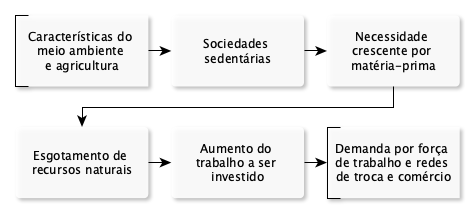
\includegraphics[width=\textwidth]{./TABELA.png}  
\end{figure}
%\begin{absolutelynopagebreak}
%\end{absolutelynopagebreak}
%\hfill
%\thispagestyle{empty}
% \caption{Frontispício da primeira edição.}

\medskip
Neste sentido, ele parece antecipar em parte a
ecologia cultural de Julian Steward.\footnote{1902--1972.}

Schmidt analisa as formas de organização social dos aruaques com relação às atividades econômicas e às diferenciações sociais internas. A expansão dos aruaques seria menos populacional, no sentido de grupos inteiros se deslocarem para novos territórios, mas, sobretudo, caracterizada por dominação social e cultural. A necessidade de manter suas comunidades sedentárias desencadearia processos de procura por ampliação da força de trabalho não mais encontrada na própria sociedade, porém a incorporação de membros de outras se daria tanto por subjugação militar quanto, majoritariamente, por influências culturais exercidas de forma lenta e sutil, de modo que a expansão dos aruaques possa ser chamada \textit{sociocultural}. Neste sentido, serão analisadas as mais diversas formas, relatadas nas etnografias consultadas, de relações entre aruaques e não aruaques: conflitos interétnicos com o objetivo de roubar ou escravizar mulheres e crianças, casamentos por rapto ou \textit{raubehe}, dominação militar, alianças políticas, casamentos interétnicos pacificamente regularizados, adoções, visitas, festas, rituais, trocas de objetos, etc. Até o ritual da couvade é interpretado neste sentido: no caso de residência pós"-nupcial uxorilocal, sua função seria socialmente agregativa por conseguir vincular genros à unidade doméstica do sogro (aruaque).

Além desses mecanismos de dominação, Schmidt apresenta uma série de
outros que podiam ser rotulados de \textit{ideológicos} num sentido quase
marxista: mitos, determinados rituais e magias. Até as artes plásticas
serão interpretadas como tendo essa função social.

\section{Inserir um nome aqui}

Sua teoria sobre o caráter e as causas da expansão aruaque nas
terras baixas da América do Sul tem pouco a ver com as teorias
migratórias da época por identificar e explicitar diversos fatores
sociais e econômicos. Desse modo, ele conseguiu apresentar uma teoria
própria de mudança cultural, ao mesmo tempo funcionalista e dinâmica.
Ela pode ser melhor caracterizada como uma teoria de sobreposição
social e cultural engatada com algum tipo de teoria de dependência
\textit{avant le nom}: os aruaques transformam em dependentes outros
grupos ou povos antes independentes por contribuir à satisfação das
necessidades econômicas destes e, ao mesmo tempo, de si mesmos. Com
as palavras do autor, ``Correspondem então, por um lado, o instinto de
ganho e, por outro lado, o instinto de subjugação''.\footnote{No original alemão: \textit{Es entsprechen sich also der Erwerbstrieb auf der einen Seite und der
Unterwerfungstrieb auf der anderen Seite}.} Um vocabulário
ultrapassado, sim, mas indicador de uma teoria original.

Schmidt lança uma crítica contundente\footnote{No sexto capítulo.} contra o padre Wilhelm
Schmidt e a \textit{doutrina dos círculos culturais}, em particular contra a
aplicação dessa teoria para explicar a diversidade das culturas
indígenas sul"-americanas.\footnote{Schmidt, 1913.} Tanto os círculos culturais\footnote{Em alemão, \textit{Kulturkreise}.} quanto as camadas culturais\footnote{Em alemão, \textit{Kulturschichten}.} não teriam nenhuma base empírica. O caráter
especulativo do \textit{difusionismo} austro"-alemão é confrontado com a própria
teoria de mudanças culturais, inspirada, por sua vez, na teoria de
mudança cultural do sociólogo Alfred Vierkandt.\footnote{1867--1953.} Vierkandt distinguiu \textit{bens culturais},\footnote{Em alemão, \textit{Kulturgüter}.} \textit{essenciais} e \textit{não essenciais}, o que explica
sua utilidade para o modelo de mudança cultural esboçado por Schmidt
para os processos de \textit{aruaquização}.\footnote{Em alemão, \textit{Aruakisierung}.}

Por estes motivos aqui brevemente apresentados, \textit{Die Aruaken} é um clássico da 
etnologia sul"-americanista que ainda
vale a pena ler. Escrito num dos períodos mais terríveis da história
humana, não parece à toa o apelo ao leitor no desfecho do livro: que este perceba como 
mudanças culturais podem ser alcançadas sem
imposições violentas. Teria sido uma lembrança tímida de um humanista
acerca dos objetivos desastrosos do Império que levariam o país à derrota
militar e ao colapso econômico um ano depois?

\section{Sobre esta edição}

A ideia de publicar uma tradução de \textit{Die Aruaken} surgiu alguns
anos atrás, em uma conversa sobre obras clássicas da tradição etnológica alemã com enfoque sul"-americanista que ainda não existiam em português. Optamos pelo livro
de Schmidt devido a sua importância no contexto da etnologia
indígena das terras baixas da América do Sul. Inicialmente imaginamos
publicar apenas a tradução junto a uma apresentação e uma nota
explicativa do tradutor, mas com o tempo percebemos que uma
contextualização tanto biográfica quanto científica ajudaria os leitores
a conhecer outros aspectos da obra e de seu autor.

Por isso, ficamos muito gratos ao saber que um colega da Universidade de Göttingen, Michael Kraus, especialista em história da antropologia e um dos melhores conhecedores da história da etnologia alemã, disponibilizou um artigo inédito em português. Seu artigo contextualiza não só o livro traduzido, mas toda a obra de Schmidt como parte de uma tradição na etnologia alemã e, ao mesmo tempo, explica suas particularidades e seu caráter excepcional. Além disso, o texto ajuda a desnudar, indiretamente, toda uma série de narrativas reducionistas e simplórias que circulam em muitas grades curriculares nacionais de graduação e pós"-graduação sobre autores clássicos como Schmidt, suas visões dos \textit{outros} e suas maneiras de conduzir pesquisas de campo. Em outras palavras: o texto de Kraus merece ser lido não só por pessoas interessadas na obra de Schmidt.

Também optamos por anexar dois breves textos biográficos, ambos de
1951, ou seja, publicados pouco tempo depois do falecimento de Schmidt:
o obituário redigido com muita sensibilidade por Herbert Baldus e um
texto quase desconhecido de Paulo de Carvalho Neto sobre os últimos ---
tristes --- dias de Schmidt. Max Schmidt faleceu em condições de miséria
total depois de ter dedicado, de modo incansável, uma vida inteira à
etnologia.

\section{Sobre Schmidt}

Aliás, a biografia acadêmica de Schmidt parece ser bem %pouco?
conhecida e apenas a descoberta de documentos inéditos pode lançar novas luzes sobre
ela. Para quem gostaria de conhecê"-la em maiores detalhes, existem três
fontes principais: a \textit{autobiografia}, anotada e redigida por Carvalho
Neto,\footnote{Schmidt, 1955.} a sinopse biográfica de Susnik, de 1991, com
resenhas de todos os trabalhos de Schmidt, e, sobretudo, o artigo
recente de Bossert e Villar, de 2019. Pouco se sabe, no entanto, sobre a
biografia não acadêmica de Schmidt, porque sua personalidade sempre foi
descrita como muito reservada e tímida. Ao que parece, Baldus não tinha
conhecimento nem do casamento com uma paraguaia chamada Mari, em 1914,
nem de alguns dilacerantes reveses trágicos da vida de Schmidt, posto que
não os menciona no obituário.

Chega a ser um milagre que Schmidt tenha conseguido finalizar sua tese de
doutorado durante a Primeira Guerra Mundial, já que em maio de 1917
falecera sua mãe e, em 24 de julho do mesmo ano, sua filha única, Grete.
Tudo indica que sua esposa já o tinha abandonado quando essas duas
tragédias se abateram sobre ele. Estas informações biográficas, não
mencionadas no artigo de Bossert e Villar, apenas ficaram
conhecidas com a pesquisa documental criteriosa de Petschelies\footnote{2019, p.
521--529.} no espólio de Theodor Koch"-Grünberg, arquivado na
Philipps"-Universität Marburg.

Um dos aspectos mais enigmáticos de sua vida certamente são os motivos
de sua surpreendente renúncia aos cargos acadêmicos na Alemanha, em
1929, e sua emigração, primeiro para o Brasil e depois para o Paraguai.
Bossert \& Villar\footnote{Páginas 23--24.} avançaram mais do que outros autores
por também levantar a hipótese de que Schmidt poderia ter tomado sua
decisão por pressentir o clima tóxico para a etnologia alemã com o
nazismo em ascensão na parte final da República de Weimar. Além disso,
parece que nem existiam mais vínculos familiares que poderiam ter
atrasado ou impedido sua emigração.

Seja como for, comparando as biografias de etnólogos alemães do período
do final do século \textsc{xix} até a década de 1940, chamam a atenção dois
aspectos semelhantes nas vidas de Schmidt e do antropólogo brasileiro de
origem alemã Curt Nimuendajú:\footnote{1883--1945.} a opção radical pela
emigração, sem as menores intenções de retorno, e a renúncia total a
qualquer conforto material. Como se sabe, as obras dos dois tiveram
impactos muito diferentes, e Nimuendajú continua ser considerado uma
figura pioneira na constituição da etnologia indígena no Brasil e da
antropologia brasileira em geral, enquanto Schmidt, ainda que citado
principalmente entre especialistas, a publicação de suas
fotografias por Bossert e Villar, com apoio do ator Viggo
Mortensen, certamente tenha ajudado a chamar a atenção para sua obra.

Pensamos que está na hora de fazer uma nova leitura, devidamente
contextualizada, de um autor que não mereceria ficar esquecido e cuja
obra \textit{Os aruaques} continua a ser um clássico, visto que esteve à
frente de sua época.

% \begin{bibliohedra}
% \tit{BOSSERT}, Federico \& \textsc{villar}, Diego. \textit{Hijos de la selva. La
% fotografía etnográfica de Max Schmidt -- Sons of the Forest. The
% Ethnographic Photography of Max Schmidt.} Santa Monica, \textsc{ca}: Perceval
% Press, 2013.

% \titidem. Una vida antropológica: biografía de Max Schmidt.
% \textit{Bérose -- Encyclopédie internationale des histoires de
% l'anthropologie.} Paris: \textsc{iiac"-lahic}, \textsc{cnrs}/Ministère de la Culture, 2019.
% (disponível em:
% \textless{}hedra.com.br/r/N3C\textgreater{};
% acesso em 15/04/2020)

% \tit{HILL}, Jonathan \& \textsc{santos-granero}, Fernando. \textit{Comparative
% Arawakan Histories: Rethinking Language Family and Culture Area in
% Amazonia\textit{.}} Urbana, Chicago: University of Illinois Press, 2002.

% \tit{PETSCHELIES}, Erik. \textit{As redes da etnografia alemã no Brasil
% (1884--1929).} (Tese de doutorado) Programa de Pós"-Graduação em
% Antropologia Social (\textsc{ppgas}), Universidade Estadual de Campinas,
% Campinas, 2019.

% \tit{SCHMIDT}, Max. Autobiografia de Max Schmidt. \textit{Revista de
% Antropologia,} São Paulo, v.\,3, n. 2, p. 115--124, 1955. (disponível em:
% \textless{}hedra.com.br/r/P4n\textgreater{};
% acesso em 15/04/2020)

% \tit{SCHMIDT}, Wilhelm, S.V.D. Kulturkreise und Kulturschichten in Südamerika.
% \textit{Zeitschrift für Ethnologie}, Berlin, n. 45, p. 1014--1030,
% 1913.

% \tit{SUSNIK}, Branislava. \textit{Prof. Dr.\,Max Schmidt: su contribución
% etnológica e su personalidad.} Asunción: Museo Etnográfico Andrés
% Barbero, 1991.

% \tit{VIERKANDT}, Alfred. \textit{Die Stetigkeit im Kulturwandel: Eine
% soziologische Studie}. Leipzig: Duncker \& Humblot, 1908.
% \end{bibliohedra}